\begin{frame}{CART -- Functionality}

\footnotesize

% \maketag{Supervised} 
\maketag{regression} \maketag{classification}
\maketag{Nonparametric} \maketag{White-box} \maketag{Feature selection}

\medskip

\highlight{General idea}
\begin{itemize}
  \item Starting from root node containing all data, perform repeated 
  \textbf{binary splits}, thereby subsequently dividing input space into $T$ 
  \textbf{rectangular partitions} $Q_t$
  \begin{itemize}
    \item In each step, find \textbf{optimal split} (feature-threshold 
    combination) $\rightarrow$ greedy search
    \item Assign same response $c_t$ to all observations in terminal region 
    $Q_t$
  \end{itemize}
  \item Splits based on node \textbf{impurity}, equivalently interpretable as 
  \textbf{ERM}
  % \item Unless interrupted, splitting continues until each observation ends up 
  % in its own leaf node $\rightarrow$ \textbf{control complexity}
\end{itemize}

\medskip
 
\highlight{Hypothesis space} ~~
$\Hspace = \left\{ \fx: \fx = \sum_{t = 1}^T c_t \I(\xv \in Q_t) 
\right\}$

\medskip

\begin{minipage}[b]{0.5\textwidth}
  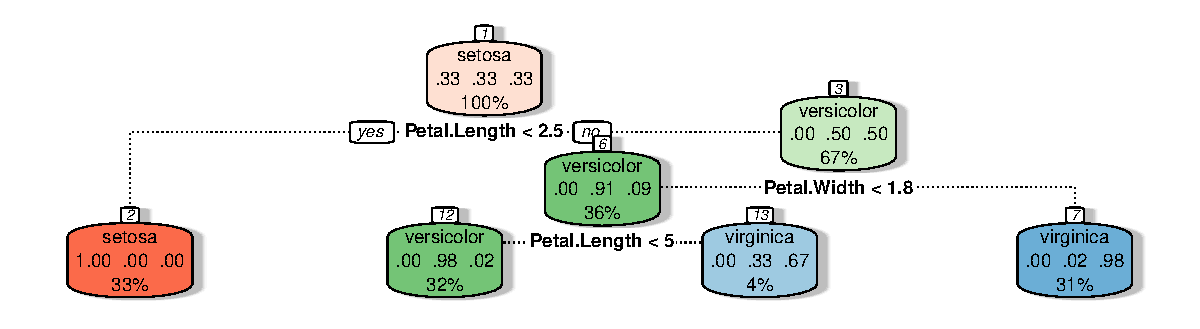
\includegraphics[width=\textwidth]{../slides/trees/figure/cart_treegrow_32} \\
  \tiny{Classification tree for \texttt{iris} data after 3 splits}
\end{minipage}
\begin{minipage}[b]{0.49\textwidth}
  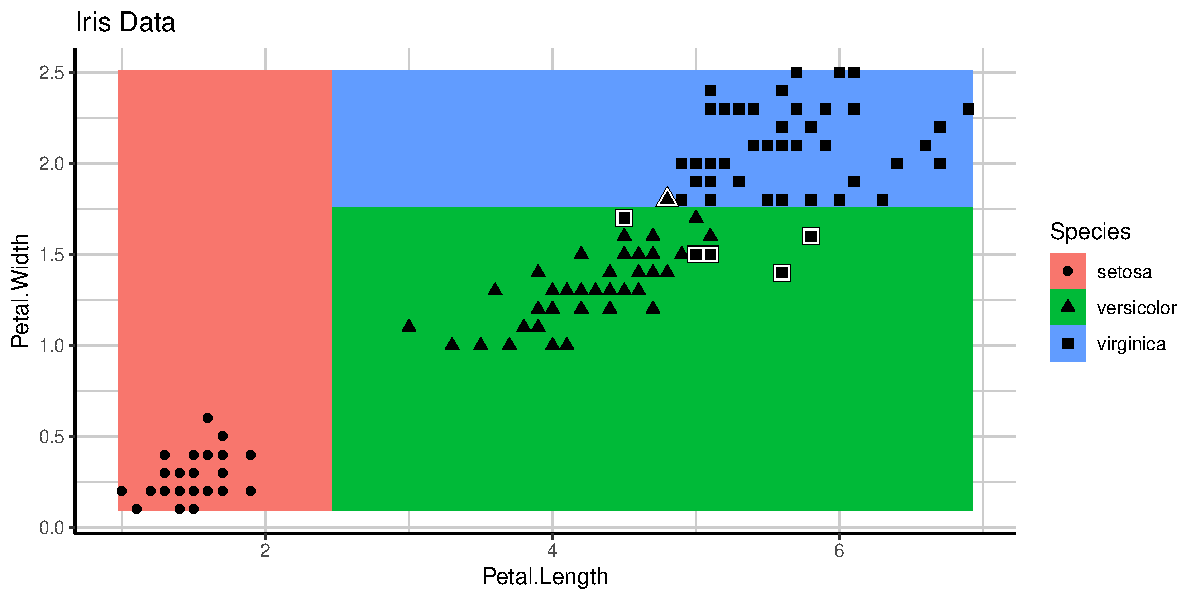
\includegraphics[width=\textwidth]{
  ../slides/trees/figure/cart_splitcriteria_1} \\
  \tiny{Corresponging prediction surface with axis-aligned boundaries}
\end{minipage}%

\end{frame}

% ------------------------------------------------------------------------------

\begin{frame}{CART -- Functionality}

\footnotesize

\highlight{Empirical risk} \\

\begin{itemize}
  \item Calculated for each potential terminal node $\Np_t$
  of a split
  \item In general, compatible with arbitrary losses -- typical choices:
  \begin{itemize}
    \footnotesize
    \item $g$-way classification:
    \begin{itemize}
      \footnotesize
      \item \textbf{Brier score} ~~
      $\risk(\Np_t) = \sum\limits_{(\xv,y) \in \Np_t} \sumkg \left( \I(y = k)
      - \pikx \right)^2$ ~~ $\rightarrow$ \textbf{Gini} impurity
      \item \textbf{Bernoulli} loss ~~
      $\risk(\Np_t) = \sum\limits_{(\xv,y) \in \Np_t} \sumkg \I(y = k) \cdot
      \log(\pikx)$ ~~ $\rightarrow$ \textbf{entropy} impurity
    \end{itemize}
    \item Regression: \textbf{quadratic} loss ~~
    $\risk(\Np_t) = \sum\limits_{(\xv,y) \in \Np_t} (y - c_t)^2$
  \end{itemize}
\end{itemize}

\medskip

\highlight{Optimization}

\begin{itemize}
  \item \textbf{Exhaustive} search over all split candidates, choice of 
  risk-minimal split
  \item In practice: limit number of candidates, use tricks to avoid 
  combinatorial explosion
\end{itemize}

\medskip

\highlight{Hyperparameters} ~~ \textbf{Complexity}, i.e., 
number of leaves $T$ (controlled indirectly, see \textit{Implementation}) 

\end{frame}

% ------------------------------------------------------------------------------

\begin{frame}{CART -- Pro's \& Con's}

\begin{columns}[onlytextwidth]
  \begin{column}{0.5\textwidth}
    \highlight{Advantages}
    \footnotesize
    \begin{itemize}
      \positem \textbf{Easy} to understand \& visualize
      \positem Highly \textbf{interpretable}
      \positem Built-in \textbf{feature selection}
      \positem Applicable to \textbf{non-numerical} features
      \positem Automatic handling of \textbf{missings} 
      \positem \textbf{Interaction} effects between features naturally included, 
      even of higher orders
      \positem \textbf{Fast} computation and good scalability
      \positem High \textbf{flexibility} (custom split criteria or leaf-node 
      prediction rules)   
    \end{itemize}
  \end{column}
  \begin{column}{0.5\textwidth}
    \highlight{Disadvantages}
    \footnotesize
    \begin{itemize}
      \negitem Rather \textbf{poor generalization} when used stand-alone 
      \negitem High \textbf{variance/instability}: strong dependence on training 
      data
      \negitem Substantial risk of \textbf{overfitting}
      \negitem Not well-suited for modeling \textbf{linear} relationships
      \negitem \textbf{Bias} toward features with \textbf{many categories}
    \end{itemize}
  \end{column}
\end{columns}

\vfill

\small

\conclbox{Simple, good with feature selection and highly interpretable, but not 
the most performant learner}

\end{frame}

% ------------------------------------------------------------------------------

\begin{frame}{CART -- Practical hints}

\footnotesize

\highlight{Complexity control}

\begin{itemize}
  \item Unless interrupted, splitting continues until we have one observation per 
  leaf node (costly + overfitting)
  \item Limit tree growth via
  \begin{itemize}
    \item \textbf{Early stopping:} stop growth prematurely \\ $\rightarrow$ hard 
    to determine good stopping point before actually trying all combinations
    \item \textbf{Pruning:} grow to large size and cut back in risk-optimal 
    manner
  \end{itemize}
\end{itemize}

\medskip

\highlight{Bagging / boosting} ~~ 
As CART are highly \textbf{instable} predictors on their own, they are typically 
used as base learners in bagging (random forest) or boosting ensembles.

\medskip

\highlight{Implementation}
\begin{itemize}
  \item \textbf{R:} \texttt{mlr3} learners \texttt{LearnerClassifRpart} / 
    \texttt{LearnerRegrRpart}, calling \texttt{rpart::rpart()}
  \item \textbf{Python:} \texttt{DecisionTreeClassifier} / 
  \texttt{DecisionTreeRegressor} from package \texttt{scikit-learn}
  \item Complexity controlled via tree depth, minimum number of observations 
  per node, maximum number of leaves, minimum risk reduction per split, ...
\end{itemize}

\end{frame}
